
% ページフォーマットの指定
\documentclass[twocolumn]{jsarticle}

  % 外部パッケージの導入
  % 引用
  \usepackage{cite}
  % 画像の出力
  \usepackage[dvipdfmx]{graphicx}
  
  % 画像元のパスの追加
  \graphicspath{{figure/}}
  
  % 文書本体の記述
  \begin{document}
  \title{プログレスレポート}
  \date{\today}
  \author{森健一郎\\配布対象:安藤先生}
  
  \maketitle
  
  \section{研究目的}
  プロセッサ・チップ上には,ホット・スポットと呼ばれる単位面積あたりの電力が大きい場所が存在する.ホット・スポットは,そうでない場所と比べて温度上昇が激しいため,プロセッサの故障を引き起こす可能性が高い.~\cite{Weste2010,Monsieur2001,Khan2010,Black1969,Viswanath2000}従って,ホット・スポットを生成する回路の消費電力を低下させる必要がある.

  ホット・スポットを生成する回路の1つに,発行キュー(IQ:issue queue)がある.IQ のサイズはプロセッサの世代が進むごとに大きくなっており,より深刻なホット・スポットとなっている.従って,IQ の電力削減に対する要求は非常に大きい.
  
  IQ の中で最も電力を消費するのは,タグ比較の回路である.タグ比較は,発行幅分のディスティネーション・タグとすべてのソース・タグで行われるため,電力効率が非常に悪い.そこで本研究では,ディスティネーション・タグとソース・タグの下位ビットが等しい命令についてのみ比較器を動作させることにより,動作する比較器の数を減少させ電力を削減する方法を提案する.

  提案手法は,次のように実現する.IQ を複数のセグメントに分割し,第 n セグメントには,第 1 ソース・タグの下位ビットが n である命令のみをディスパッチする.そして,ウェイクアップのタグ比較の際には,ディスティネーション・タグの下位ビットが,自身に割り当てられた命令の第1ソース・タグの下位ビットと等しいセグメントのみ,比較器を動作させてタグ比較を行う.この方法により,第1ソース・タグについての比較器の動作回数を「1/セグメント数」に減少させることができる.

  提案手法における欠点として,セグメントが詰まることによる性能低下が挙げられる.あるセグメントに空きがない状態で,そのセグメントにディスパッチされる命令が現れた場合を考える.この場合,他のセグメントにディスパッチすることはできないため,該当のセグメントに空きが出るまでディスパッチを停止する必要があり,これは性能低下に繋がる.本研究では,この欠点に対する対応策を考え,性能低下が許容できる範囲内に収まるようにする必要がある.

  また,その他の欠点として,第2ソース・タグの比較器の動作回数は削減できないことなどが挙げられる.これらの欠点に対しても十分に検討し,提案手法における電力削減及び性能の変化について評価を行う.

  \section{経過}

  \subsection{前回の経過}
  \begin{itemize}
    \item ROB のサイズによる提案手法への影響の調査
    \item Last Tag Prediction の実装及び評価
  \end{itemize}
  \subsection{今回の経過}
  \begin{itemize}
    \item Last Tag Prediction(LTP) に GHB 方式を実装
    \item セグメントを第 2 ソースタグに基づき更に分割するサブ・セグメントを実装
    % \item 容量効率を重視したモードと比較削減を重視したモードを適切に切り替える SWITCH 方式を実装
  \end{itemize}    

  \section{活動報告: g-share 方式の LTP の実装及び評価}
  前回のレポートで,両方のタグがレディでない場合に,より遅くにレディとなるタグを予測して,そのタグを発行キューのセグメント化された方に入れるという Last Tag Prediction(LTP)を実装した.しかし,前回レポート時点では LTP を構成するテーブルのインデクスに単純な PC のみを用いていたため,予測精度が低くなっていた. 

  LTP が提案された論文~\cite{ernst2002} によると,テーブルのインデクスには,PC とグローバル分岐履歴の XOR を用いる g-share 方式が採用されている.そこで今回は,  g-share 方式を実装し,予測精度の測定を行った.g-share 方式では,図~\ref{fig:ltp_gshare}のように,テーブルのインデクスを PC の下位ビットとグローバル分岐履歴の XOR によって計算する.なお,グローバル分岐履歴は分岐予測ミスのリカバー時に正しい履歴に書き換えるようにしている.また,グローバル分岐履歴は論文 ~\cite{ernst2002} に基づき 8 bit としている.

  g-share 方式の LTP をシミュレータに実装し,予測精度の評価を行った.評価環境とその結果を以下に示す.

  \begin{figure}[ht]
    \centering
    \includegraphics[width=0.99\hsize]{ltp_ghb.pdf}
    \caption{Last Tag Predictor(g-share)}
    \label{fig:ltp_gshare}
  \end{figure}

  \begin{table}[htb]
    \caption{プロセッサの基本構成}
    \footnotesize
    \center
      \begin{tabular}{l|l} \hline \hline
       Pipeline width & 8 instructions wide for each of \\
       & fetch, decode, issue, and commit \\
       Reorder buffer & (Small) 256 entries \\
       & (Medium) 320 entries \\
       & (Huge) 1024 entries \\
       IQ & 128 entries \\
       Load/Store queue & 128 entries \\
       Physical registers & (Small) 256(int) + 256(fp) \\
       & (Medium) 320(int) + 320(fp) \\
       & (Huge) 1024(int) + 1024(fp) \\
       Branch prediction & 12-bit history 4K-entry PHT gshare \\
       & 2K-set 4-way BTB \\
       & 10-cycle misprediction penalty \\
       Function unit & 4 iALU, 2 iMULT, \\
       &  3 FPU, 2 LSU \\
       L1 D-cache & 32KB, 8-way, 64B line \\
        & 2-cycle hit latency \\
       L1 I-cache & 32KB, 8-way, 64B line \\
        &  2-cycle hit latency \\
       L2 cache & 2MB, 16-way, 64B line \\
        & 12-cycle hit latency \\  
       Main memory & 300-cycle latency \\
       & 8B/cycle bandwidth \\ 
       Prefetch & stream-based,32-stream tracked,  \\ 
       & 16-line distance, 2-line degree, \\
       & prefetch to L2 cache \\ \hline
    \end{tabular}
    \label{tab:base_config}
  \end{table}

  \subsection{評価環境}
  評価環境について説明する.シミュレータには SimpleScalar をベースに修正を加えたものを使用した.表\ref{tab:base_config}にプロセッサ構成を示す. Reorder buffer 及び Physical registers の構成として,Small, Medium,Huge の 3 つのモデルを想定している.これまでの測定では Small モデルを用いていたが,以降の測定では,基本として Medium モデルを使用して行う.これは, ROB が詰まることを防ぎ,発行キューの評価を適切なものにするためである. 
  
  測定ベンチマークには,SPEC CPU 2017 ベンチマークのうち,int 系 9 本と fp 系 9 本の計 18 本を使用した.ベンチマークの測定区間は,プログラムの先頭から 16G 命令をスキップした後の 100M 命令である.

 \begin{figure*}[ht]
    \centering
    \includegraphics[width=0.99\hsize]{ltp_ghb_acc.pdf}
    \caption{LTP の予測精度}
    \label{fig:ltp_ghb_acc}
  \end{figure*}

  \subsection{評価結果}
  g-share 方式の LTP による予測精度について,図~\ref{fig:ltp_ghb_acc}に測定結果を示す.横軸がベンチマーク,縦軸が予測精度を表す.また,各ラベルは LTP のエントリ数及びインデクスの方法が PC か g-share 方式かを表している.

  同図より,g-share 方式での測定精度は,エントリ数が同じ場合で PC の 2\% 程度しか向上しておらず,大きな向上は見られないことが分かる.これはどのベンチマークでも同様である.従って, g-share 方式での LTP の有効性は PC 方式の場合とほぼ同程度であるといえる.

  ただ,論文~\cite{ernst2002} によると,g-share 方式による LTP の予測精度は 8 から 9 割程度とされているのに対して,今回の測定では 7 割程度の精度にとどまっている.評価環境が異なるので一概には言えないが,もしかすると論文で想定されている予測方法と今回の実装で異なる部分がある可能性がある.もう少し改良の余地がないか探ろうと思う.

  なお,g-share 方式の場合の性能及び比較回数の削減率に関しては,前回レポートで示した PC を用いた場合の LTP と優位な差が見られなかったため,本レポートでは省略している.

  \section{活動報告:サブ・セグメントの実装と評価}
  現在の提案手法の欠点として,第 1,2 ソース・レジスタがともにレディでない場合に,第 2 ソース・レジスタでのタグ比較を削減できないことが挙げられる.この欠点を解消するため,サブ・セグメント方式を提案する.

  \subsection{サブ・セグメント方式の概要}
  サブ・セグメントは図~\ref{fig:sub_segment} のように, 第 1 ソース・タグ値に基づいて分割された各セグメント(図中の黒枠)を,第 2 ソース・タグ値に基づいて更に分割する手法である.図の例では,4 つに分割したセグメントを,それぞれさらに 2 つのサブ・セグメントに分割している.
  
  なお以降の説明では,第 1 ソース・タグ値に基づく通常のセグメントを,サブ・セグメントと対比してメイン・セグメントと呼ぶ.また,図~\ref{fig:sub_segment}中の(a,b)で表される番号は,a がメイン・セグメントの番号を,b がサブ・セグメントの番号を表している.

  \begin{figure}[ht]
    \centering
    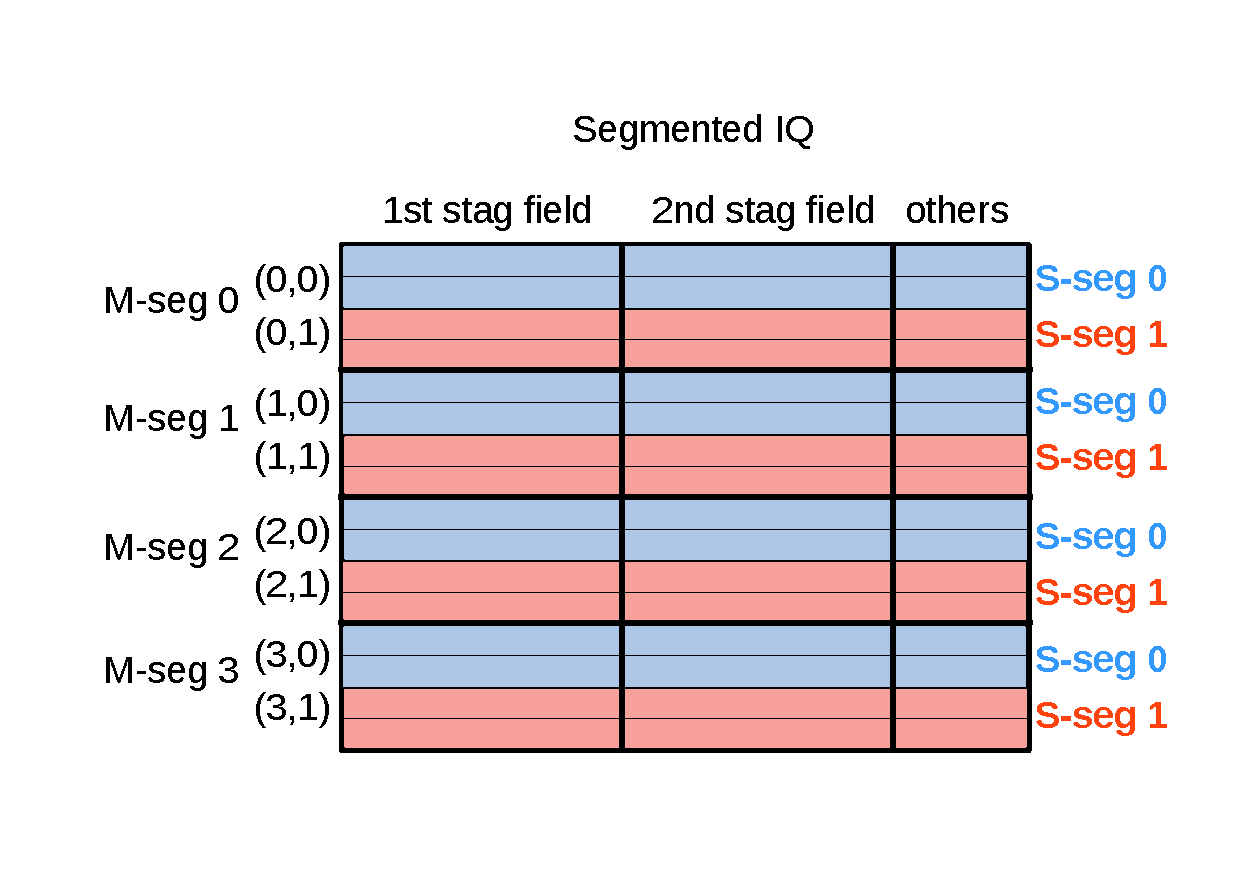
\includegraphics[width=0.99\hsize]{sub_segment.pdf}
    \caption{サブ・セグメントを実装した IQ}
    \label{fig:sub_segment}
  \end{figure}

  \subsubsection{サブ・セグメント方式におけるディスパッチ}
  サブ・セグメント方式におけるディスパッチについて,ソース・レジスタのレディ状況ごとに例を用いて説明する.以下の例で用いる発行キューは,メイン・セグメント数が 4,サブ・セグメント数が 2  (図~\ref{fig:sub_segment}と同様)であるとする.

  \paragraph{1: reg1,reg2 ともにレディでない場合}
  r2 = r6 + r3 という命令について考える.r6,r3 はともにレディでないとする.第 1 ソース・タグより,メイン・セグメントは2(=6 \% 4)となる.また,第 2 ソース・タグより,サブ・セグメントは1(= 3 \% 2)となる.したがってディスパッチするセグメントは (2, 1)のセグメントとなる. 
  \paragraph{2: reg1 がレディで reg2 がレディでない場合}
  r2 = r6 + r3 という命令について考える.r6 はレディで r3 はレディでないとする.第 1 ソース・レジスタはレディであるため,メイン・セグメントはどこでも良い.しかし第 2 ソース・レジスタはレディでないため. サブ・セグメントは 1(= 3 \% 2) である必要がある.従って,(0, 1)(1, 1)(2, 1)(3,1)のいずれかのセグメントに割当を行う.
  \paragraph{3: reg1 がレディなく reg2 がレディである場合}
  r2 = r6 + r3 という命令について考える.r6 はレディでなく r3 はレディであるとする.第 1 ソース・レジスタはレディでないため,メイン・セグメントは2(=6 \% 4)となる.一方で第 2 ソース・レジスタはレディであるため, サブ・セグメントはどこでも良い.従って,(2, 0)(2, 1)のいずれかのセグメントに割当を行う.
  \paragraph{4: reg1,reg2 ともにレディである場合}
  どのセグメントにディスパッチしても良い(セグメント・フレキシブル).

  なお,今回の測定では,ディスパッチ可能なセグメントが複数ある場合(2,3,4の場合),もっとも空き数の多いセグメントにディスパッチするようにしている.

  \subsubsection{サブ・セグメント方式におけるタグ比較}
  サブ・セグメント方式における第 2 ソース・タグの比較は,ディスティネーション・タグの下位ビットがサブ・セグメント番号と同じ場合のみ行われる.これによって,これまでの提案手法では削減ができなかった第 2 ソース・タグのタグ比較も削減することができる.
  
  \subsubsection{SWAP 方式へのサブ・セグメントの適応}
  サブセグメントは,SWAP 方式にも適応が可能である.基本的なディスパッチの動作は上述の説明と同じで,スワップを行う際には reg1 のタグを第 2 ソース・タグとして扱い,reg2 のタグを第 1 ソース・タグとして扱う.どのタイミングでスワップを行うかは,以前のレポートで説明したものと同様である.

  \subsection{評価}
  サブ・セグメント方式を適応した場合の提案手法による性能変化と比較回数の削減率を測定した.今回の測定では,提案手法のうちスワップを行わない通常の方式(NORMAL)と,スワップを行い出来るだけ容量効率を低下させない方式(SWAP\_CONSERVATIVE : SWAP\_CONS)について測定を行った.測定結果に関して評価を行う.評価環境は~\ref{tab:base_config}と同様である.

  \begin{figure*}[ht]
    \centering
    \includegraphics[width=0.99\hsize]{IPC_normal_subsegment.pdf}
    \caption{サブ・セグメントによる性能変化(NORMAL)}
    \label{fig:IPC_normal_subsegment}
  \end{figure*}

  \begin{figure*}[ht]
    \centering
    \includegraphics[width=0.99\hsize]{acc_normal_subsegment.pdf}
    \caption{サブ・セグメントによる IQ 占有率の変化(NORMAL)}
    \label{fig:acc_normal_subsegment}
  \end{figure*}

  \begin{figure*}[ht]
    \centering
    \includegraphics[width=0.99\hsize]{comp_normal_subsegment.pdf}
    \caption{サブ・セグメントによる比較回数削減率(NORMAL)}
    \label{fig:comp_normal_subsegment}
  \end{figure*}


  \subsubsection{NORMAL の評価}
  サブ・セグメント方式を実装した NORMLA における 性能変化,発行キューの占有率,比較回数の削減を図~\ref{fig:IPC_normal_subsegment},~\ref{fig:acc_normal_subsegment},~\ref{fig:comp_normal_subsegment}に示す.各図におけるラベルNormal(a,b)は,メイン・セグメントの分割数が a,サブ・セグメントの分割数が b である NORMAL 方式であることを表す.
  
  まず,図~\ref{fig:IPC_normal_subsegment}の性能変化と図~\ref{fig:acc_normal_subsegment}の占有率について考える.図~\ref{fig:IPC_normal_subsegment}の横軸はベンチマークとその平均を,縦軸は通常の発行キュー(age 論理)に対する相対性能を表す.図~\ref{fig:acc_normal_subsegment}の横軸はベンチマークとその平均を,縦軸は発行キューの占有率を表している.ラベルの Base は通常の発行キュー(age 論理)の際の占有率である.
  
  図より,(32,1) 及び (16,2) ではいくつかのベンチマーク(cactuBSSN や lbm など)で性能が低下していることが分かる.これは図~\ref{fig:acc_normal_subsegment}の占有率を見て分かるとおり,分割するセグメント数が多すぎて大幅に占有率が低下していることが原因であると考えられる.

  (32,1)と(16,2)に関して詳しく見てみると,性能が低下しているすべてのベンチマークで(32,1)よりも(16,2)の性能低下が小さくなっていることが分かる.これは,(32,1)よりも(16,2)のほうが占有率の低下が小さいためであると考えられる.従って,トータルのセグメント数が同じ場合((32,1)と(16,2)はどちらも 32 個のセグメントに分割されている)は,サブ・セグメントを用いたほうが占有率の低下が抑えられるため,結果として性能低下を小さくできるということがわかった.
  
  次に,図~\ref{fig:comp_normal_subsegment}の比較回数削減に関して考える.図の横軸はベンチマーク及びその平均,縦軸は比較回数の削減率を表す.図より,サブ・セグメントを利用すると,利用しない場合に対して 10 \% 程度削減率が増加することが分かる.従って,第 2 ソース・レジスタがレディでない場合も有効的にタグ比較の削減が行えていることが分かる.

  \begin{figure*}[ht]
    \centering
    \includegraphics[width=0.99\hsize]{IPC_swap_subsegment.pdf}
    \caption{サブ・セグメントによる性能変化(SWAP\_CONSERVATIVE)}
    \label{fig:IPC_swap_subsegment}
  \end{figure*}

  \begin{figure*}[ht]
    \centering
    \includegraphics[width=0.99\hsize]{acc_swap_subsegment.pdf}
    \caption{サブ・セグメントによる IQ 占有率の変化(SWAP\_CONSERVATIVE)}
    \label{fig:acc_swap_subsegment}
  \end{figure*}

  \begin{figure*}[ht]
    \centering
    \includegraphics[width=0.99\hsize]{comp_swap_subsegment.pdf}
    \caption{サブ・セグメントによる比較回数削減率(SWAP\_CONSERVATIVE)}
    \label{fig:comp_swap_subsegment}
  \end{figure*}

  \subsubsection{SWAP\_CONSERVATIVE の評価}
  サブ・セグメント方式を実装した SWAP\_CONSERVATIVE における 性能変化,発行キューの占有率,比較回数の削減を図~\ref{fig:IPC_swap_subsegment},~\ref{fig:acc_swap_subsegment},~\ref{fig:comp_swap_subsegment}に示す.各図の表現は NORMAL の場合と同様である.

  まず,図~\ref{fig:IPC_swap_subsegment}の性能変化に関して考える.SWAP\_CONSERVATIVE は容量効率を重視した方式であるため,基本的に大きな性能低下は見られない.
  
  次に図~\ref{fig:acc_swap_subsegment}の占有率に関して見てみると,NORMAL の場合と比較して占有率の低下は小さいことが分かる.また,(32,1)と(16,2)を比較してみても,多くのベンチマークで大きな違いはみられない.従ってSWAP\_CONSERVATIVE の場合には,サブ・セグメントを利用することによる占有率の変化は小さいと言える.

  次に,図~\ref{fig:comp_swap_subsegment}の比較回数の削減に関して考える.こちらも NORMAL の場合と同様に,サブ・セグメントを利用したほうがより多く削減できていることがわかり,サブ・セグメントが有効に働いていると言える.

\subsubsection{サブ・セグメント方式のまとめ}
  以上の結果により,サブ・セグメントを利用すると,
  \begin{itemize}
    \item NORMAL の場合は占有率の低下を抑えることができ
    \item 比較回数を10\%程度多く削減できる
  \end{itemize}
  ことがわかった.従って,サブ・セグメントは非常に有効な手段であると言える.


  % \section{活動報告:SWITCH 方式の実装と評価}
  % 以前のレポートで,スワップ方式において,タグ比較の削減を重視する SWAP\_AGGRESIVE 方式と,容量効率の低下を防ぐことを重視する SWAP\_CONSERVATIVE 方式の 2 種類の方式を提案した.この 2 つの方式には,表~\ref{tab:swap_nature}のようなトレードオフの関係がある.

  % \begin{table}[htb]
  %   \caption{スワップ方式のトレードオフ}
  %   \footnotesize
  %   \center
  %     \begin{tabular}{c|c|c}  \hline
  %      方式 & 容量効率 & タグ比較削減 \\ \hline
  %       AGGRESIVE & × & ○ \\
  %      CONSERVATIVE & ○ & × \\ \hline
  %   \end{tabular}
  %   \label{tab:swap_nature}
  % \end{table}
  
  % より積極的な削減を行いつつ,性能低下を防ぐには,これらの 2 つの方式を必要に応じて動的に切り替えて利用するとよいのではないかと考えられる.そこで今回は, SAWAP\_AGGRESIVE と SWAP\_CONSERVATIVE を動的に切り替え,より積極的にタグ比較を削減しつつ性能の低下を抑制するような SWITCH 方式を提案する.

  % \begin{figure}[ht]
  %   \centering
  %   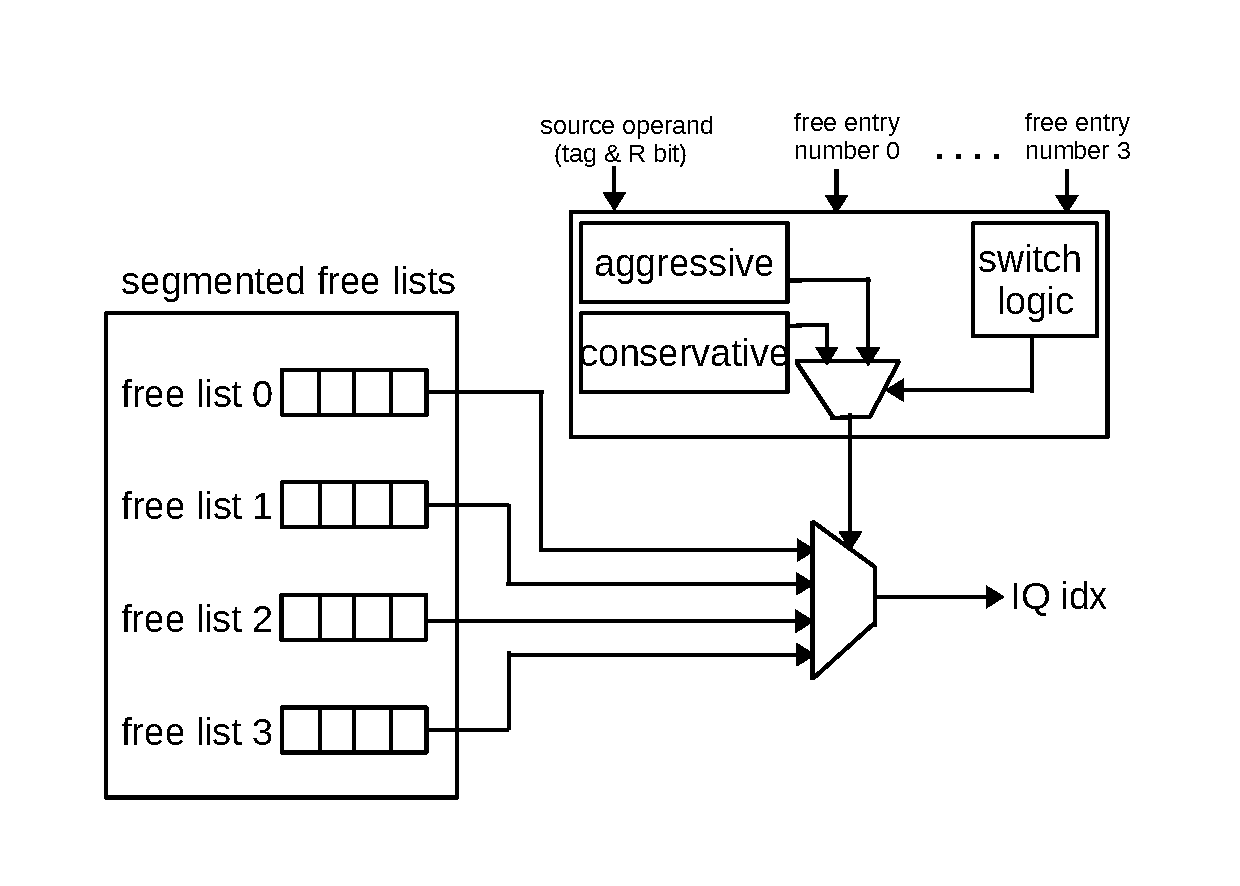
\includegraphics[width=0.99\hsize]{switch.pdf}
  %   \caption{SWITCH 方式の状態遷移図}
  %   \label{fig:switch}
  % \end{figure}

  % \subsection{SWITCH 方式の実装}
  % SWITCH 方式において重要となるのは,SWAP\_AGGRESIVE と SWAP\_CONSERVATIVE を切り替えるアルゴリズムである.つまり,発行キューの容量効率が性能に影響を与えるかどうかを判断するアルゴリズムが重要となる.

  % 論文~\cite{Kora2013}によると,発行キューの容量効率が必要となるのは,LLC キャッシュ・ミスが生じた場合である.これは発行キューの容量効率が低下すると利用可能な MLP が制限されてしまうためである.

  % そこで今回は,L2 キャッシュ・ミスを切り替えに利用するイベントとした.
  % L2 キャッシュ・ミスが生じた場合に SWAP\_AGGRESIVE からSWAP\_CONSERVATIVE へと切り替える.そして,SWAP\_CONSERVATIVE へと切り替えてからメモリ・レイテンシだけ時間が経過したら SWAP\_AGGRESIVE へと戻す.図~\ref{fig:switch}にこのアルゴリズムの状態遷移図を示す.

  % なお,この切り替えはディスパッチのアルゴリズムを切り替えるのみであるため,発行キューに大きな変更を加える必要はないと思われる.

  % \subsection{SWITCH 方式の評価}
  % SWITCH 方式を実装し評価を行った.

  \section{研究計画}
  
  \begin{itemize}
    \item HSPICE を用いた電力測定を開始する
    \begin{itemize}
      \item 現在は測定方法などを松田さんから教わり,各コードで何をやっているかの理解をしている段階
      \item ウェイクアップ論理を修正して提案手法での消費電力及び遅延を測定できるようにする
      \item フリー・リストの論理に関してはおそらく実装されていないため,実装して測定する
      \item 提案手法におけるディスパッチ時の遅延の増加が懸念されるため実装し測定したい
    \end{itemize}
    \item LTP の予測精度向上
    \item サブ・セグメント方式のチューニング
  \end{itemize}
  
  \section{関連文献: MLP-Aware Dynamic Instruction Window Resizing
for Adaptively Exploiting Both ILP and MLP~\cite{Kora2013}}
本論文では,MLPを利用できる場合発行キューのサイズを大きくし,そうでない場合には発行キューのサイズを小さく制限する手法を提案している.

一般に,IQ のサイズが大きいほど利用できるメモリ・レベル並列性(MLP) は大きくなり,キャッシュ・ミスによるメモリアクセスのレイテンシを隠蔽することができ,性能の向上につながる.しかし,すべてのプログラムにおいて MLP が利用できるわけでない. MLP が利用できない場合, IQ のサイズが大きいことが原因となり, ILP が損なわれたり,分岐命令の実行が遅れ分岐予測ミス・ペナルティが増加してしまい,性能の低下が発生する.

従って,MLP が利用できる場合には IQ のサイズを大きくし,そうでない場合にはサイズを小さく制限することが有効であると考えられる.本研究では,LLC キャッシュ・ミスが生じた際に IQ のサイズを大きくし,メモリ・アクセスに必要なサイクルが経過した後に元のサイズに戻すという方法を提案している.

通常 LLC キャッシュ・ミスは固まって発生するため,一度 LLC ミスを起こすと連続して メモリ・アクセスが発生するため,この間に発行キューのサイズを大きくしておけばより MLP を利用できる.

本論文によると,この提案手法により平均で 21\% の性能向上を達成している.

\subsection{自身の提案手法への応用}
自身の提案手法における SWAP\_AGGRESIVE と SWAP\_CONSERVATIVE は,容量効率と比較回数の削減の間にトレードオフの関係がある.そこで,この関連論文のように容量効率が重要なときのみ SWAP\_CONSERVATIVE を用いて,そうでない場合には SWAP\_AGGRESIVE を用いれば,より積極的な削減を達成しつつ性能低下を抑制できるのではないかと考えられる.これは,提案手法の応用方法として検討すべき今後の課題と言える.
  
  
  % 参考文献
  \bibliographystyle{../Config/andolab2} 
  \bibliography{../Config/ref}
  
  \end{document}
  